\documentclass[10pt,twocolumn]{article}

\usepackage{times}
\usepackage{spverbatim}
\usepackage[swedish]{babel}
\usepackage[utf8]{inputenc}
\usepackage{listings}
\usepackage[toc,page]{appendix}
\usepackage{graphicx}
\usepackage{mathtools}
\usepackage{float}
\usepackage{algorithm}
\usepackage{algpseudocode}
\usepackage[margin={2.45cm, 2.45cm}]{geometry}
\renewcommand\appendixname{Bilagor}
\renewcommand\appendixpagename{Bilagor}
\usepackage[compact]{titlesec}
\titlespacing{\section}{0pt}{*2}{*2}
\raggedbottom
\sloppy

\title{Lab 3\\ \emph{OpenMP}}

\author{Martin Söderén \\ marso329, 9009291098 }

\date{\today}

\begin{document}

\maketitle

\clearpage

\section{Introduction}

The problem consists of solving a stationary heat conduction problem using OpenMP on a shared memory computer. The problem consists of a grid of points in a 2D configuration. All points have a initial value and for each time step each points temperature changes depending on the average temperature of the surrounding points. This keeps on going until the solution converges. 
\section{Method}
The grid is implemented as a array of arrays of doubles. The grid is split up row wise into chunks. The number of chunks is equal to the number of points in each column divided by the number of threads. So the number of rows in a chunk is equal to the number of threads. In each iteration the chunks are calculated one after another from top to bottom in the grid. Each time a chunk is calculated one thread takes one row each, synchronize and then writes back the data to the grid. But before the write back the last row is stored so that it can be used in the next chunk since that depends on data in the last row of that chunk. 

\begin{algorithm}[H]
\caption{Stationary heat conduction}
\label{alg:Master}
\begin{algorithmic}
\Procedure{HEAT}{}
\If{Master}
\State Init grid
\EndIf
\For{maxiter}
\State Error=0 (shared)
\State copy first row into copy\_before
\State Calculate numberOfChunks
\For{numberOfChunks}
\State calculate the start row for this chunk
\If{Master}
\State copy\_after=last row of chunk 
\EndIf
\State Synchronize using omp barrier
\State calculate which row to work on
\State temp\_error=0.0
\For{each element in row}
\State calculate new temp
\State calculate temp\_error
\If{local\_error$>$ temp\_error}
\State temp\_error=error
\EndIf
\EndFor
\State Synchronize using omp barrier
\State access critical section using omp\_set\_lock
\If{if temp\_error$>$error}
\State error=temp\_error
\EndIf
\State Write back data to grid
\State leave critical section using omp\_unset\_lock
\If{Master}
\State Switch copy\_before and copy\_after
\EndIf
\EndFor
\If{error$<$tolerance}
\State exit
\EndIf

\EndFor
\EndProcedure
\end{algorithmic}
\end{algorithm}



\subsection{Design}
The whole program runs in parallel because at first the parallel part was started in the iteration loop and that meant that in each iteration new threads had to be created which took a lot of time and had a huge impact on performance so instead the program runs in parallel from top to bottom. More or less all threads runs the same loop that is synchronized before the calculation and before the write back.

\section{Result}
The stationary heat conduction calculation scales fairly well up to 11 cores. With 11 cores there is reduction of calculation time 2.5 lower than the time with a single core. With more cores there is hardly any difference in speed.  The times were measured with a grid of 1000x1000 points. With a larger grid there might be a more significant change since each core can do more job in each chunk. The reason for the poor increase in performance can be because of the critical section which all threads needs to access to write back the error of chunk.
\begin{figure}[H]
	\begin{center}
		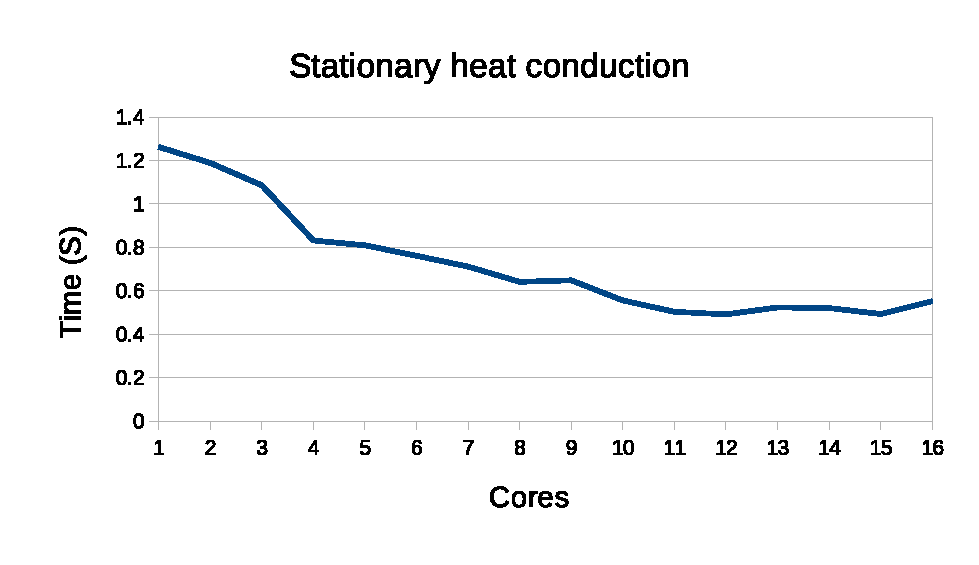
\includegraphics[scale=0.5]{figurer/heat.eps}
	\end{center}
	\caption{Times heat conduction calculation with a 1000x1000 grid}
\end{figure}


\newpage

\onecolumn
\appendix
\section{lapsolvomp.c} \label{app:blur}
\lstinputlisting[language=c]{../lapsolvomp.c}

\end{document}
